\documentclass[main]{subfiles}
\begin{document}

%@@@@@@@@@@@@@@@@@@@@@@@@@@@@@@
% Main Topics: Passive Membrane Properties I - 11.10.2018
% Lecturer: Valerio Mante
% author: Vanessa Leite - base document from benelot/eth-intro-to-neuroinformatics-summary

\section{Passive (Cable) Membrane Properties}

\subsection{Biophysics of the membrane}
\begin{itemize}
\item Membrane separates in and out. It is an insulator/capacitor.
\item Ionic pumps: $[ion]_{in} \neq [ion]_{out}$
\item Selective ion channels
\end{itemize}

Those three factors give us the reversal (resting) potential: $E_{ion}$.

\subsection{Basic electronics}
\begin{itemize}[noitemsep,nolistsep]
	\item Ohm's Law: $V = I \cdot R$
	\item Kirchoff's Current Law (KCL): The sum of all currents entering and leaving any node in a circuit is zero.
	\item Kirchoff's Voltage Law (KVL): The sum of all voltages around a closed loop is equal to zero.
\end{itemize}

\subsection{Ion channel replacement circuit}
\begin{itemize}[noitemsep,nolistsep]
	\item Ion channel is equal to resistance.
	\item Ion gradient is equal to battery.
	\item Cell membrane is equal to capacitor.
	\item Conductivity $S=\frac{1}{R}$.
	\item Ion resistance is $R = V/I$.
	\item Ion conductivity is $\gamma = g_L = I/V$.
	\item Outward current for an ion is $I_m=g_L(V-E_L)$.
	\item If the concentration of an ion on one side is raised (with a corresponding molecule of opposite charge) and the membrane is permeable for this ion, then the side which has a higher concentration gets more negative, because the ions go to the other side, leaving behind uncompensated negative charges.
\end{itemize}
\begin{figure}[H]
	\centering
	\scalebox{0.7}{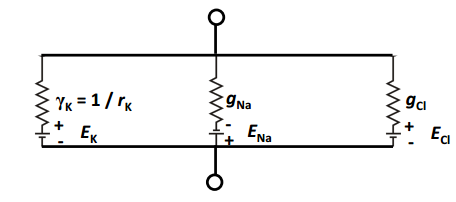
\includegraphics{ion_channel_circuit_01.png}}
\end{figure}
\begin{figure}[H]
	\centering
	\scalebox{0.7}{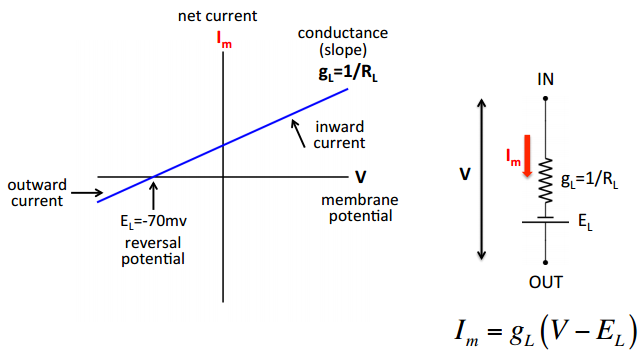
\includegraphics{current_voltage_01.png}}
\end{figure}

We say conductance is ohmic when we have passive properties, thus, $I = g \cdot V$.
Different channel types have different resting potential. For example, AMPA/NMDA (excitatory) have $E_{rev} \approx 0 mV$. GABA A and GABA B (inhibitory) have $E_{rev} \approx -65 mV$ and $-90 mV$, respectively.

Synapses are injecting (externeal) current.
Assume dendrite are passive cables that just conduct current (this is a simplification, we are discarding, for instance, backprop action potential and dendrite computation.). This way, we have three models:
\begin{itemize}
\item Single compartment model: voltage has only temporal dependency $V = V(t)$.
\item Cable equation: depends on time and location (analytical solutions) $V = V(x,t)$.
\item Multicompartment model: (numerical solutions) $V = V(x,t)$.
\end{itemize}

Those approaches offer a trade-of between realism and complexity.

\subsection{Single-compartment model}

\paragraph{Assumptions, configuration}
\begin{itemize}[noitemsep,nolistsep]
	\item Assume isopotential $V = V(t)$: holds locally
	\item Spherical membrane.
	\item $I_e$ is an injected current.
	\item $I_C$ is the capacitive current, charges the membrane.
	\item There is also a leak current $I_m = g_m(V-E_R)$.
	\item $[ion]_{in} = [ion]_{out} \rightarrow V_{rest} = 0$, equivalent to $v(t) = V(t) - E_R$
\end{itemize}

\paragraph{Membrane as electrical circuit}

At $t = 0$ an external current arrives, the membrane is charged and some current leak. At $t > 0$, $I_e > I_m$, i.e., the injected current is bigger than the leak current (some current is charging the membrane). At $t = \infty$,  we reach the equilibreium, $I_e = I_m$ and $I_C$ = 0, with the membrane completely charged, all the current that enters, leave.

\begin{itemize}[noitemsep,nolistsep]
	\item $I_e  - I_m = I_C$ and $I_m=g_m(V-E_R)$
	\item $C = \frac{Q}{V} \rightarrow CV = Q \rightarrow C\frac{dV}{dt} = \frac{dQ}{dt} = I_C$
	\item $I_e - gm \cdot v(t) = C_m \cdot \frac{dV(t)}{dt}$
	\item Membrane time-constant: $\tau_m = R_m \cdot C_m$
	\subitem depends on the resistances and the capacitors. Usual range from 10-100 ms.
	\item Larger current due to spatial summation.
	\item Less depolarization with small resistance (larger area).
\end{itemize}

\begin{figure}[H]
	\centering
	\begin{subfigure}[b]{0.3\textwidth}
		\centering
		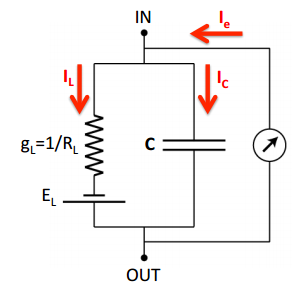
\includegraphics[width=\textwidth]{membrane_circuit_01.png}
	\end{subfigure}%
	~
	\begin{subfigure}[b]{0.5\textwidth}
		\centering
		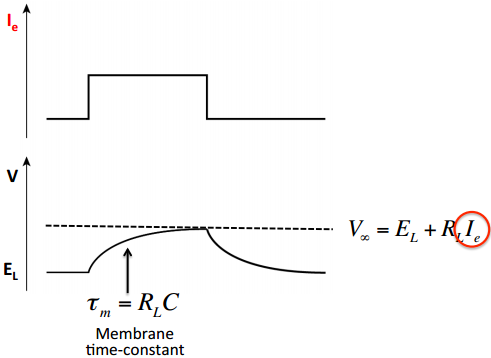
\includegraphics[width=\textwidth]{membrane_circuit_02.png}
	\end{subfigure}
	\caption{$R_L = R_m$, $E_L = E_m$, $g_L = g_m$, $I_L = I_m$}
\end{figure}

\subsubsection{Steady-state}
$R_m$ as input resistance.

$V_\infty = R_m \cdot I_e + E_m$: steady-state, i.e., voltage doesn't change anymore ($\frac{dV}{dt}=0$).

$V_\infty$ increases if $R_m$ increases (less leak) or $I_e$ increases (more input)

\paragraph{Consequences}
Two neurons with the same concentration of channels, differing only regarding the size: the smaller neuron will have more resistance, thus, for the same amount of current ($I_e$) it will have smaller voltage change ($R_{small neuron} \rightarrow V^{small}_\infty$ and $R_{large neuron} \rightarrow V^{large}_\infty$). Thus, $R_m = \frac{r_m}{area}$.

Two neurons, one myelinated and another unmyelinated. The myelinated has less resistance thus it needs less current input ($I_e$) to achieve the same voltage change.

\subsubsection{Time-dependency}
$\tau_m$ is the memory of cell $\approx 10$ to $100 ms$. Neuron forgets after $\tau$.

\paragraph{several solutions}
\[V(t) = E_m + R_m \cdot I_e + (V(0) - E_m - R_m \cdot I_e) \epsilon^{\frac{-t}{\tau_m}}\]

\paragraph{single solution}
\[v(t) = v_\infty+(v(0)-v_\infty)e^{-\frac{t}{\tau_m}}\]
for $v = V - E_m$

\paragraph{Consequences}
Consider $I_{e1} \rightarrow V_1(t)$ and $I_{e2} \rightarrow V_2(t)$, then, $V_1(t) + V_2(t)$ is result of $I_{e1} + I_{e2}$.

\subparagraph{Spatial summation} 
Simultaneous inputs ($\delta t = 0$) sum linearly.
If $I_e \rightarrow k \cdot I_e$ then $V_\infty \rightarrow k \cdot V_\infty$.

\subparagraph{Sequential inputs}
Sequential inputs sum if $\delta t < \tau_m$.
It is quite fuzzy, very different from computers.

\subparagraph{Constant inputs}
When achieve the threshold, it generates an action potential and right after, reset it. This is knowing as Integrate and Fire neuron.
$r_{isi} = \frac{1}{t_{isi}} \approx \frac{E_m - V_{th} + R_m I_e}{\tau_m \cdot (V_{th} - V_{reset})}$

\subparagraph{idealized synapse}
if $I_e > 0$ then $V > E_m$ leading to EPSP (depolarization). 
if $I_e < 0$ then $V < E_m$ leading to IPSP (hyperpolarization).

\subsubsection{Equivalent electrical circuit}

\paragraph{Neuron}
\begin{figure}[H]
	\centering
	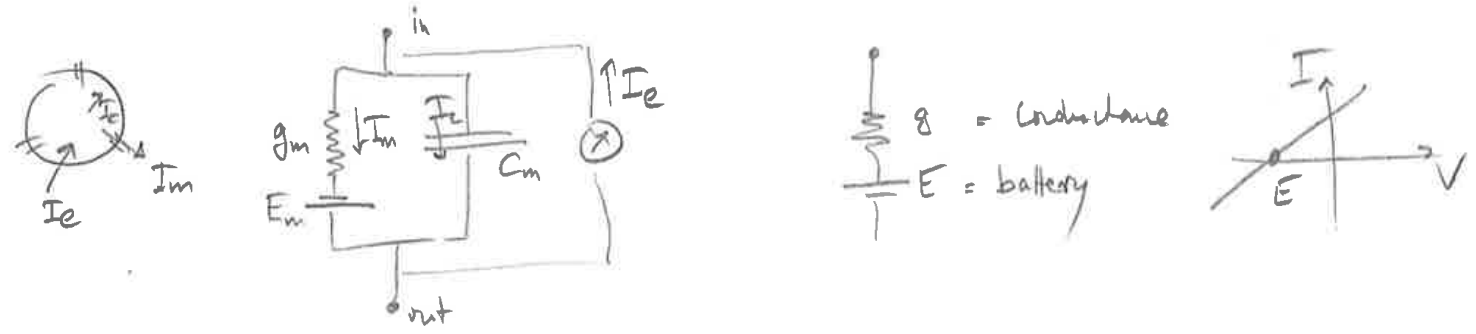
\includegraphics[width=\textwidth]{electrical_circuit_neuron.png}
\end{figure}

\paragraph{Adding synapse}

\begin{figure}[H]
	\centering
	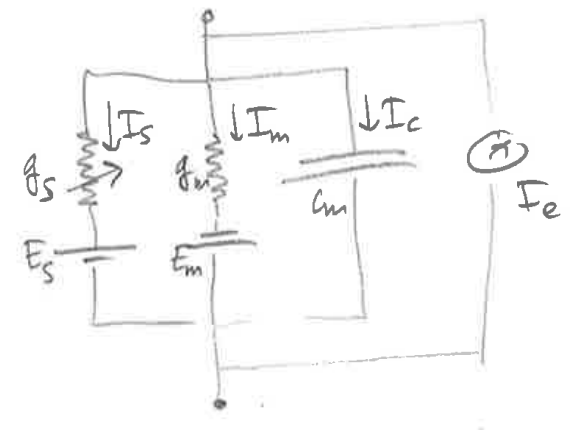
\includegraphics[width=\textwidth]{electrical_circuit_neuron_synapse.png}
\end{figure}

$I_C + I_m + I_s = I_e$
$C_m \frac{dV}{dt} + g_m (V - E_m) + g_s(V - E_s) = I_e$

%\begin{itemize}[noitemsep,nolistsep]
%	\item Equilibrium at $I_L=I_S$
%	\item $V_\infty = \frac{g_LE_L+g_SE_S}{g_L+g_S}$
%	\item $\tau_m = \frac{C}{g_L+g_S}$
%\end{itemize}

\subsection{The cable equation}
\[c_m\frac{\partial V}{\partial t} = \frac{1}{2ar_L}\frac{\partial}{\partial x}(a^2\frac{\partial V}{\partial x})-i_m+i_e\]
\begin{figure}[H]
	\centering
	\scalebox{0.7}{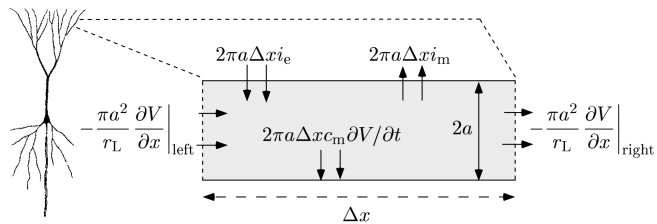
\includegraphics{cable_equation_01.png}}
\end{figure}

\subsubsection{Infinite cable}
\begin{figure}[H]
	\centering
	\scalebox{0.7}{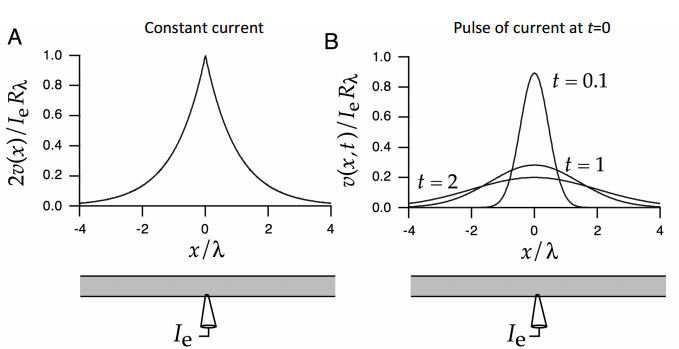
\includegraphics{cable_equation_02.png}}
\end{figure}
\begin{itemize}[noitemsep,nolistsep]
	\item $v(x) = \frac{I_eR_\lambda}{2}\exp(-\frac{|x|}{\lambda})$
	\item $R_\lambda=\frac{r_m}{2\pi a\lambda} = \frac{r_L\lambda}{\pi a^2}$
	\item $\lambda = \sqrt{\frac{ar_m}{2r_L}}$ sets the scale for the spatial variation in the membrane potential.
	\item $\lambda$ is the electronic length, or how far the signal travels.
	\item $\tau_m = r_mc_m$ sets the scale for the temporal variation in the membrane potential.
	\item $v(x,t) = \frac{I_eR_\lambda}{\sqrt{4\pi\lambda^2t/\tau_m}}\exp(-\frac{\tau_mx^2}{4\lambda^2t})\exp(-\frac{t}{\tau_m})$
	\item $a$ is the radius of the axon, about $2\,\mu m$
	\item $r_m$ is the specific membrane resistance, about $1\,M\Omega\cdot mm^2$
	\item $v = V - V_{rest}$
	\item $r_L$ is the longitudinal resistance, about $1\,k\Omega\cdot mm$
	\item $I_e$ is the injected current.
	\item It follows, that increasing $R_m$ also increases $\lambda$. With better isolation, signals travel further.
	\item Increasing the diameter also increases $\lambda$.
\end{itemize}

\subsection{Level of approximation}
\begin{itemize}[noitemsep,nolistsep]
	\item A neuron can be represented by a variable number of discrete compartments.
	\item Compartments represent a region, each with a single membrane potential.
	\item The connections between compartments have resistive couplings.
\end{itemize}

\subsection{Hodgkin-Huxley Equations}
\begin{itemize}[noitemsep,nolistsep]
	\item Model that describes how action potentials in neurons are initiated and propagated.
	\item $n$ and $m$ are probabilities for a gate to be open.
	\item $h$ is the probability that an open channel is not blocked.
	\item The gating variables have a voltage dependence.
	\item $\bar{g}$ values are the maximum conductance possible.
	\item There is no inactivation for potassium, only for sodium.
	\item The membrane does not get locked at positive values.
	\item $\bar{g}_L$ stands for some generic leak.
	\item The functions $n_\infty(V)$, $m_\infty(V)$ and $h_\infty(V)$ determine whether gates serve to activate channels (with depolarization) or inactivate the channel (close with depolarization). $\tau_m$, $\tau_h$ and $\tau_n$ are time constants.
\end{itemize}
\[C\frac{dV}{dt}+\bar{g}_Kn^4(V-V_K)+\bar{g}_{Na}m^3h(V-V_{Na})+\bar{g}_L(V-V_L)+I_{inj}=0\]

\begin{figure}[H]
	\centering
	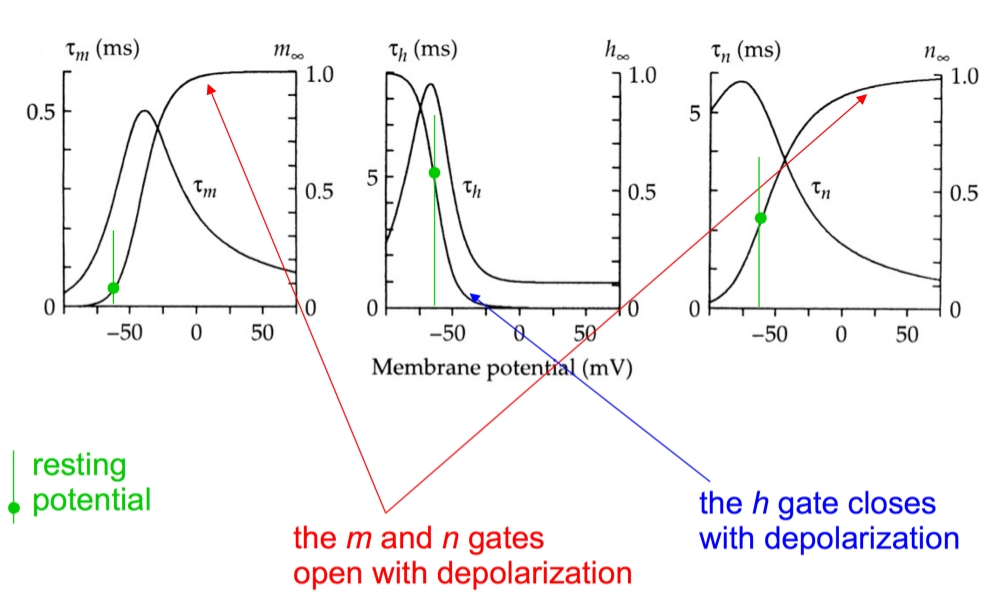
\includegraphics[scale=0.5]{5_8.jpg}
\end{figure} 
\begin{figure}[H]
	\centering
	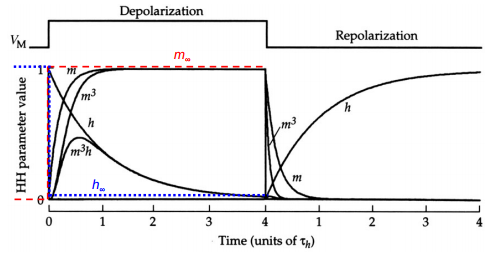
\includegraphics[scale=1.0]{depolarization_01.png}
\end{figure} 



\end{document}
